\chapter{Sort}


\section{INTRODUCTION}
List of general algorithms:
\begin{enumerate}
\item Selection sort: invariant
\begin{enumerate}
\item Elements to the left of $i$ (including $i$) are fixed and in ascending order (fixed and sorted).
\item No element to the right of $i$ is smaller than any entry to the left of $i$ ($A[i]  \leq\min(A[i+1:n])$.
\end{enumerate}
\item Insertion sort: invariant
\begin{enumerate}
\item Elements to the left of $i$ (including $i$) are in ascending order (sorted).
\item Elements to the right of $i$ have not yet been seen.
\end{enumerate}
\item Shell sort: h-sort using insertion sort.
\end{enumerate}


\section{CONTEXT}
$O(N\lg N)$ is the lower bound of comparison-based sorting; but for other contexts, we may not need $O(N \lg N)$:
\begin{enumerate}
\item Partially-ordered arrays: insertion sort to achieve $O(N)$.
\item Duplicate keys
\item Digital properties of keys: radix sort to achieve $O(N)$.
\end{enumerate}
\section{STABILITY}
Definition: a stable sort preserves the \textbf{relative order of items with equal keys} (scenario: sorted by time then sorted by location). 

Algorithms:
\begin{enumerate}
\item Stable
\begin{enumerate}
\item Merge sort
\item Insertion sort
\end{enumerate} 
\item Unstable
\begin{enumerate}
\item Selection sort
\item Shell sort
\item Quick sort
\end{enumerate}
\end{enumerate}
\textbf{Long-distance swap} operation is the key to find the unstable case during sorting. 
\begin{figure}[hbtp]
\centering
\subfloat{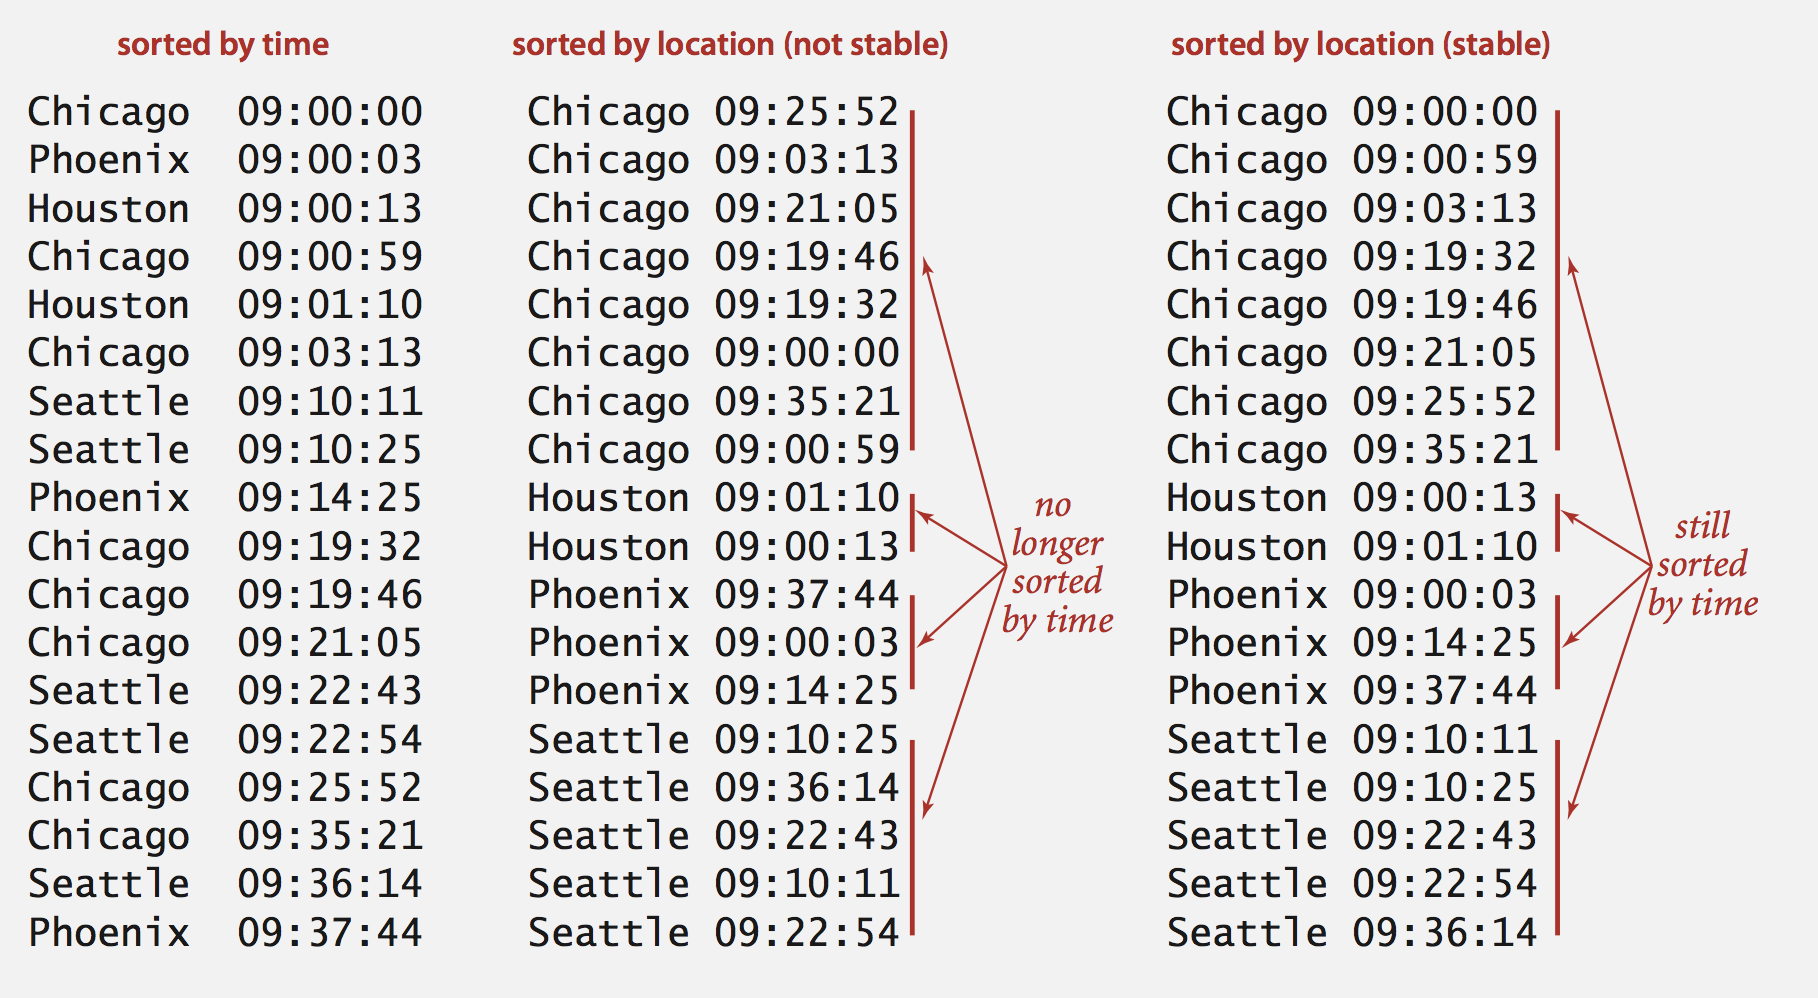
\includegraphics[scale=.60]{stable_sort}}
\caption{Stale sort vs. unstable sort}
\label{fig:trie} 
\end{figure}

